\documentclass[english]{article}
\usepackage[T1]{fontenc}
\usepackage[latin9]{inputenc}
\usepackage{geometry}
\geometry{verbose,tmargin=1in,bmargin=1in,lmargin=1in,rmargin=1in,headheight=1cm,headsep=1cm,footskip=1cm}
\usepackage{amsmath}
\usepackage{amssymb}
\usepackage{babel}
\usepackage{graphicx}
\usepackage{multicol}

\usepackage{caption}
\captionsetup{margin=10pt,font=scriptsize,justification=centering}


\newcommand{\xx}[0]{\mathbf{x}}
% Figures within a column...
\makeatletter
\newenvironment{tablehere}
{\def\@captype{table}}
{}
\newenvironment{figurehere}
{\def\@captype{figure}}
{}
\makeatother

\begin{document}
\title{Statistics of Nodal Domains in Quantum Chaotic Eigenfunctions in the Semiclassical Limit}
\author{Kyle Konrad \\
  Prof. Alex Barnett \\
  Computer Science Department \\
  Dartmouth College}
\maketitle

\begin{multicols}{2}

\section*{Goals and Definitions}

Classically, chaos is characterized by a strong dependence on initial conditions and the signatures of classical chaotic systems are well known. The classical description of a system however, becomes inaccurate for very small systems; one must instead use quantum mechanics. According to the correspondence principle, quantum systems approach classical behavior at high energies (the so called semiclassical limit), thus it is reasonable to expect some analogue of classical chaos in quantum systems, at least at high energies. It is not obvious how this might happen since quantum mechanics is an entirely linear theory and classical chaos requires nonlinearity; furthermore it is not obvious what chaos will look like in a quantum setting since classical characterizations do not apply. Over the past several decades, the field of quantum chaos has been exploring the manifestations of chaos in quantum systems and investigating numerical properties of such systems.

It has been conjectured that nodal domains in quantum chaotic eigenfunctions follow the same statistics as those of a percolation model for which exact asymptotic values can be obtained for many statisics of nodal domains \cite{bogolmony}. This thesis seeks to provide strong numerical evidence for this conjecture by collecting empirical data at previously unseen accuracy. This has proven challenging due to the difficulty of computing high energy eigenfunctions with sufficient resolution to obtain accurate nodal domain counts.


Quantum chaotic eigenfunctions area subset of solutions $u\left(\xx\right)$ of the Helmholtz equation 
\begin{eqnarray} \label{eq:helmholtz}
\left(\triangle+k^{2}\right)u\left(\xx\right) & = & 0\mbox{ for }\xx\in\Omega,\; k\in\mathbb{C} \\
u\left(\xx\right) & = & 0\mbox{ for }\xx\in\partial\Omega \nonumber
\end{eqnarray}
where $\Omega\in\mathbb{R}^2$ is a compact domain and $\triangle=\nabla^{2}=\frac{\partial^{2}}{\partial x^{2}}+\frac{\partial^{2}}{\partial y^{2}}$ is the Laplacian differential operator. Equation (\ref{eq:helmholtz}) can be derived from the time-independent Schr\"{o}dinger equation
\[
\triangle u \left(\xx\right)+k^{2}u\left(\xx\right)=V\left(\xx\right)u\left(\xx\right)\mbox{ for }\xx\in\Omega,\; k\in\mathbb{C}
\]
by using a step potential over $\Omega$ given by
\[
V\left(\xx\right)=\begin{cases}
0 & \mbox{if }\xx\in\Omega\\
\infty & \mbox{if }\xx\notin\Omega
\end{cases}
\]
Here $k$ is the wavenumber of the solution and is proportional to the inverse of the wavelength of the solution while $k^{2}$ is proportional to energy of the solution. This energy can be interpreted as the energy of a quantum wave-particle in $\Omega$ with the wavefunction $\psi\left(\xx\right)=u\left(\xx\right)$.

The particular subset of solutions of eq. (\ref{eq:helmholtz}) which comprise quantum chaotic eigenfunctions are those for which $\Omega\subset\mathbb{R}^{2}$ is a chaotic domain. For $\Omega$ to be chaotic means that a classical point particle in $\Omega$ exhibits hyperbolic dynamics, i.e., has positive Lyapunov exponent for almost all initial conditions \cite{chernov}.

It is known that these chaotic eigenfunctions of eq. (\ref{eq:helmholtz}) contain complex and irregular structures of nodal domains in the semiclassical limit, where a nodal domain $\eta\subseteq\Omega$ of an eigenfunction $u\left(\xx\right)$ containing a point $\mathbf{x_{0}}$ is defined as the largest connected subset of $\Omega$ such that $\text{sign}\left(\xx\right)=\text{sign}\left(\mathbf{x_{0}}\right)$ for all $\xx\in\eta$. Letting $\nu\left(k\right)$ be the number of nodal domains for a particular $k$, we can formulate the the following conjecture \cite{bogolmony}:

\vspace{10pt}
\noindent\emph{Conjecture:} The mean value of $\nu\left(k\right)$ tends to $0.0624\cdot N_{w}\left(k\right)$ as $k$ approaches infinity.
\label{conj:mean}
\vspace{10pt}

\noindent Here $N_{w}\left(k\right) = \frac{\text{Vol}\left(\Omega\right)k^{2}}{4\pi}$ is the number of eigenfunctions with energy less than $k^{2}$ given by Weyl's law \cite{nonnenmacher}. Time permitting, we will also investigate additional conjectures arising from the percolation model.

The percolation model can be formulated as a perturbation on a checkerboard pattern of alternating positive and negative regions. At each point in the interior of the checkerboard at the junction of four squares we perturb the checkerboard by connecting two of the diagonal regions, either positive to positive or negative to negative.

\section*{Methods}
\subsection*{Computing Eigenfunctions}
Due to the chaotic nature of the domains investigated herein, it is not possible to analytically solve the Schrodinger equation. In order to obtain eigenfunctions we therefore use numerical solutions to eq. (\ref{eq:helmholtz}), computed by a method first described by Vergini \cite{vergini} and implemented in C by Barnett \cite{barnett}. Vergini's method computes eigenfunctions on a discrete grid of points by solving the system of equations which arises from a combinations of plane wave (including evanescent plane waves) basis functions with a range of orientations of varying intensity requiring that the eigenfunction go to zero on the boundary $\partial\Omega$. Given the intensity of each plane wave satisfying the given boundary condition we compute the eigenfunction at each point by summing the plane waves giving a $O\left(mn^{2}\right)$ runtime where $m$ is the number of plane wave basis functions and $n$ is the number of grid points in the $x$-direction, which is inversely proportional to the grid spacing $\Delta x$. This computation is relatively expensive and dominates total computation time, restricting us to work with relatively coarsely sampled eigenfunctions, though we must have $\Delta x \lesssim \frac{1}{k}$ in order to resolve the smallest nodal domains which will have size on the order of the wavelength $\frac{1}{k}$.

\subsection*{Counting Nodal Domains Efficiently}
The development of efficient computational methods to identify and compute statistics of nodal domains has been the primary obstacle to verifying the conjectures of the percolation model and is the focus of this thesis. In order to obtain behavior close to the asymptotic case we work with eigenfunctions with $k \sim 10^{3}$ which have $\sim 1000$ nodal domains each. In order to collect sufficient data to obtain high accuracy statistics we will count nodal domains of $\gtrsim 10^{4}$ eigenfunctions. Nodal domains are counted from gridded data by fully exploring domains one at a time while marking grid points as explored and belonging to a particular domain. This method runs as $O\left(n^{2}\right)$ where $n$ is again the number of gridpoints in the $x$-direction and in practice is several hundred times faster than computing eigenfunctions. Because we are restricted to work with coarsely sampled eigenfunctions (as discussed above), the naive approach to counting nodal domains is not always accurate; we may have scenarios where we are unable to resolve the way in which nodal domains cross one another (Fig. \ref{fig:crossing}).

\begin{figurehere}
\centering
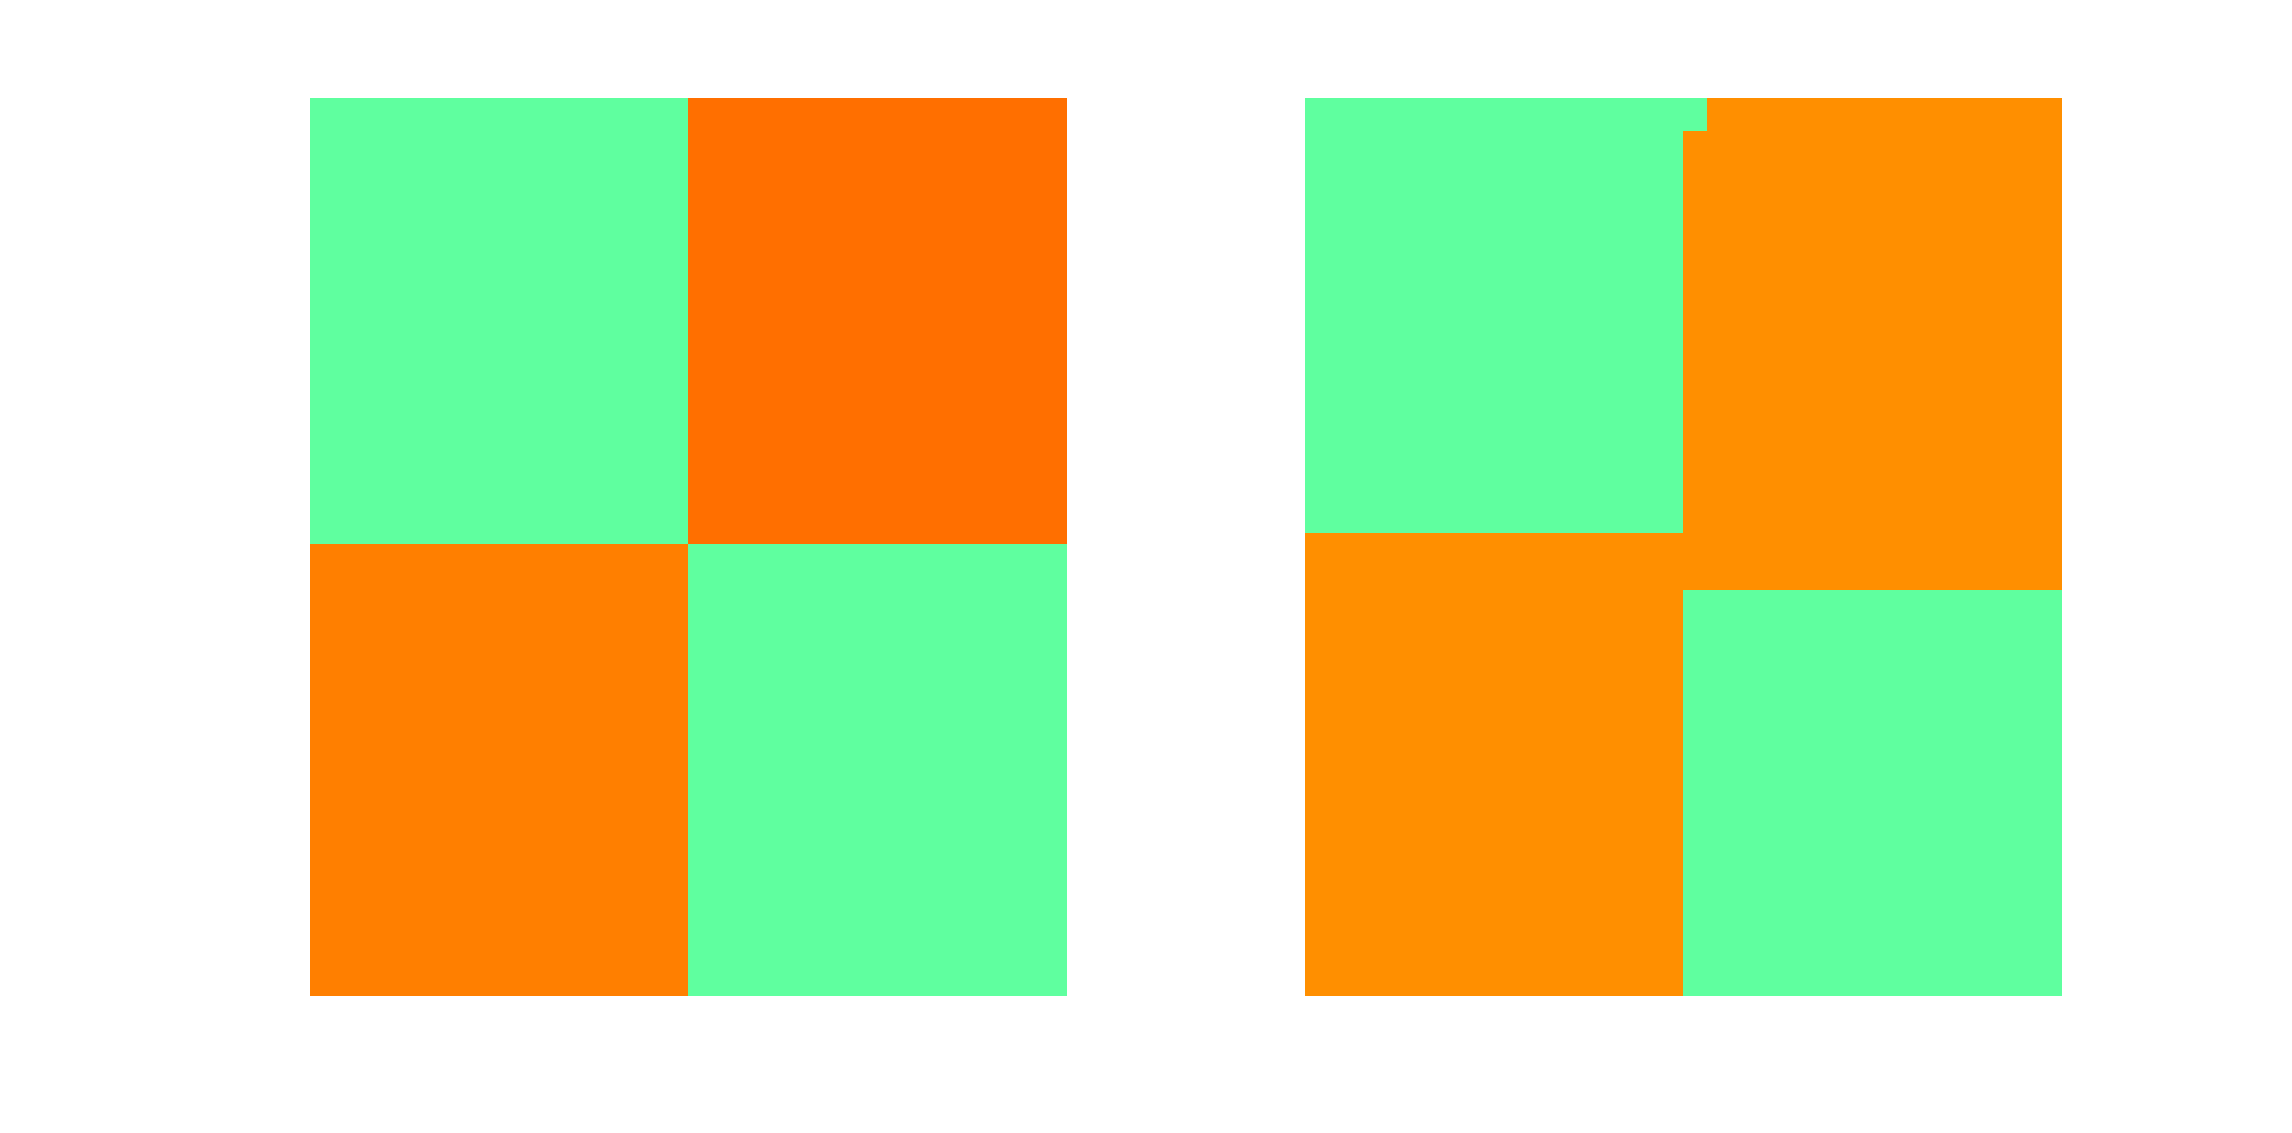
\includegraphics[width=\columnwidth]{crossing.eps}
\vspace{-30pt}
\caption{An ambiguity in nodal domain counting due to low resolution (left) and a higher resolution view (right).}
\vspace{10pt}
\label{fig:crossing}
\end{figurehere}

In order to resolve such ambiguities we can selectively interpolate our coarsely sampled eigenfunction to a much higher resolution within the small region containing the ambiguity. It can be shown that the functions

\begin{center}
$\{\xi_{n}\left(r, \theta\right)\}_{n=1}^{\infty}=1\cup\left\{ \sin\left(n\theta\right)J_{n}\left(kr\right)\right\} _{n=1}^{\infty}\cup\left\{ \cos\left(n\theta\right)J_{n}\left(kr\right)\right\} _{n=1}^{\infty}$
\end{center}
where $J_{n}\left(r\right)$ is a Bessel function of the first kind span the solution space of eq. (\ref{eq:helmholtz}). This observation allows us to interpolate by locally expanding our coarsely sampled function in terms of the basis functions $\{\xi_{n}\}_{n=1}^{\infty}$ then sampling the local surrogate function at high enough resolution to resolve the ambiguity.

\section*{Conclusion}
By developing high-precision numerical tools for counting and tracking nodal domains in quantum chaotic eigenfunctions we hope to address current conjectures of quantum chaos of interest to physicists and mathematicians. We will attempt to verify conjectures regarding the mean and variance of the number of nodal domains and possibly additional conjectures. By releasing documented source code for the tools developed herein we hope to facilitate further investigation of quantum chaotic systems in the quantum chaos community.

\bibliographystyle{plain}
\bibliography{proposal}

\end{multicols}

\end{document}
